\documentclass[11pt,class=report,crop=false]{standalone}
\usepackage[screen]{../python}

\begin{document}


%====================================================================
\chapitre{Convolution avec tensorflow/keras}
%====================================================================

\insertvideo{F4RdAcjM2cI}{partie 14.1. Reconnaissance de chiffres}

\insertvideo{ogiMe_lbvts}{partie 14.2. Reconnaissance d'images}

\insertvideo{EbcvAvFfB_c}{partie 14.3. Reconnaissance d'images - Chat vs chien}

\insertvideo{bjAWwP7h8mI}{partie 14.4. Que voit un réseau de neurones ?}



\objectifs{Nous mettons en \oe uvre ce qui a été vu dans les chapitres précédents au sujet des couches de convolution afin de créer des réseaux de neurones beaucoup plus performants.}

\index{convolution!avec tf@avec \tensorflow/\keras}

%%%%%%%%%%%%%%%%%%%%%%%%%%%%%%%%%%%%%%%%%%%%%%%%%%%%%%%%%%%%%%%%%%%%%
\section{Reconnaissance de chiffres}

On souhaite reconnaître des chiffres écrits à la main.

%--------------------------------------------------------------------
\subsection{Données}

\index{donnees@données!MNIST}

Les données sont celles de la base  MNIST déjà rencontrée dans le chapitre \og{}Python : tensorflow avec keras - partie 2\fg{}.
On rappelle brièvement que cette base contient $60\,000$ données d'apprentissage (et $10\,000$ données de test) sous la forme d'images $28\times28$ en niveau de gris, étiquetées par le chiffre attendu.
\begin{center}
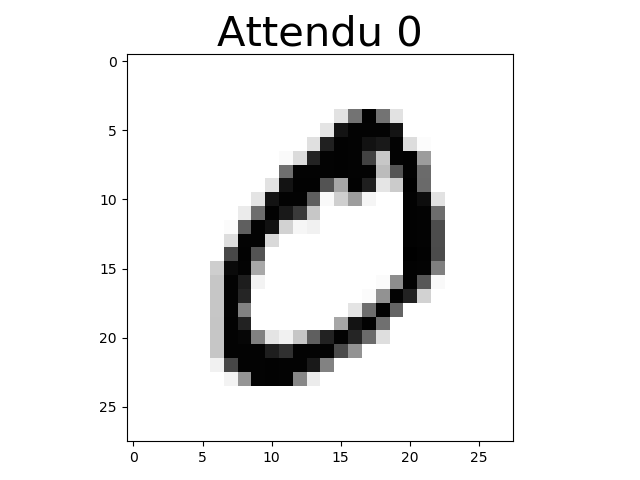
\includegraphics[scale=\myscale,scale=0.5]{figures/tfconv-chiffre-train-1}
\end{center}

Pour le besoin de la convolution, on conserve chaque image sous la forme d'un tableau $28\times 28$ ; afin de préciser que l'image est en niveau de gris, la taille du tableau \numpy{} est en fait $(28, 28, 1)$ (à comparer à la représentation d'une image couleur de taille $(28, 28, 3)$).

%--------------------------------------------------------------------
\subsection{Modèle}

On crée un réseau composé de la façon suivante :
\begin{itemize}
  \item \textbf{Première couche de convolution.} 
  Une couche formée de $32$ sous-couches de convolution. Si on note $A$ l'image de départ, chaque sous-couche est la convolution $A \conv M_i$ de $A$ par un motif $M_i$ de taille $3 \times 3$ $(i=1,\ldots,32)$. Une entrée de taille $(28,28,1)$ est transformée en une sortie de taille $(28,28,32)$.
   
  Chaque sous-couche correspond à un neurone de convolution avec $3 \times 3$ arêtes plus un biais, c'est-à-dire $10$ poids par sous-couche. Avec nos $32$ sous-couches, cela fait au total $320$ poids pour cette première couche. 
  
  \myfigure{0.4}{
  \tikzinput{fig-tfconv-cnn-01}
  } 
  
  
  \item \textbf{Seconde couche de convolution.}
  Une couche formée de $16$ sous-couches de convolution. Si on note $\mathcal{B} = (B_1,\ldots,B_{32})$ les sorties de la couche précédente, qui deviennent maintenant les entrées, alors chaque sous-couche de sortie est une convolution $\mathcal{B} \conv M'_i$ par un motif $M'_i$ de taille $3 \times 3 \times 32$. Une entrée de taille $(28,28,32)$ est transformée en une sortie de taille $(28,28,16)$.
  
  Chaque sous-couche correspond à un neurone de convolution avec $3 \times 3 \times 32$ arêtes plus un biais, soit $289$ poids par sous-couche. Avec nos $16$ sous-couches, cela fait un total de $4 624$ poids pour cette seconde couche.
  
  \myfigure{0.4}{
  \tikzinput{fig-tfconv-cnn-02}
  } 
  
  \item \textbf{Aplatissement.}
  Chaque sortie de taille  $(28,28,16)$ est reformatée en un (grand) vecteur de taille $12\,544$ ($= 28 \times 28 \times 16$). Il n'y a aucun poids associé à cette transformation : ce n'est pas une opération mathématique, c'est juste un changement du format des données.
  
  \myfigure{0.4}{
  \tikzinput{fig-tfconv-cnn-03}
  } 
    
  
  \item \textbf{Couche dense.}
  C'est une couche \og{}à l'ancienne\fg{} composée de $10$ neurones, chaque neurone étant relié aux $12\,544$ entrées. En tenant compte d'un biais par neurone cela fait
  $125\,450$ ($= (12\,544+1) \times 10$) poids pour cette couche.
  
  \myfigure{0.4}{
  \tikzinput{fig-tfconv-cnn-04}
  }   

  
  \item \textbf{Bilan.} Il y a en tout $130\,394$ poids à calculer.
  
\end{itemize}


Voici l'architecture complète du réseau.

\myfigure{0.35}{
\tikzinput{fig-tfconv-cnn-05}
} 

On résume l'architecture du réseau par des blocs, chaque bloc représentant une transformation.
\myfigure{0.5}{
\tikzinput{fig-tfconv-bloc-01}
}  

%--------------------------------------------------------------------
\subsection{Programme}

\begin{lstlisting}
import numpy as np
import matplotlib.pyplot as plt
from tensorflow import keras
from tensorflow.keras import optimizers
from tensorflow.keras.models import Sequential
from tensorflow.keras.layers import Dense, Conv2D, Flatten

### Partie A - Création des données
from tensorflow.keras.datasets import mnist
from tensorflow.keras.utils import to_categorical

(X_train_data,Y_train_data),(X_test_data,Y_test_data) = mnist.load_data()

N = X_train_data.shape[0]  # 60 000 données

X_train = np.reshape(X_train_data, (N,28,28,1))
X_test = np.reshape(X_test_data, (X_test_data.shape[0],28,28,1))

X_train = X_train/255  # normalisation
X_test = X_test/255

Y_train = to_categorical(Y_train_data, num_classes=10)
Y_test = to_categorical(Y_test_data, num_classes=10)

### Partie B - Réseau de neurones
modele = Sequential()

# Première couche de convolution : 32 neurones, motif 3x3, activ. relu
modele.add(Conv2D(32, kernel_size=3, padding='same', activation='relu',
                      input_shape=(28,28,1)))

# Deuxième couche de convolution : 16 neurones
modele.add(Conv2D(16, kernel_size=3, padding='same', activation='relu'))

# Aplatissage 
modele.add(Flatten())

# Couche de sortie : 1O neurones
modele.add(Dense(10, activation='softmax'))

# Descente de gradient
modele.compile(loss='categorical_crossentropy',
               optimizer='adam',
               metrics=['accuracy'])

print(modele.summary())

# Calcul des poids
modele.fit(X_train, Y_train, batch_size=32, epochs=5)

### Partie C - Résultats
score = modele.evaluate(X_test, Y_test, verbose=0)
print('Test loss:', score[0])
print('Test accuracy:', score[1])
\end{lstlisting}


%--------------------------------------------------------------------
\subsection{Explications}

Une couche de convolution est ajoutée avec \tensorflow/\keras{} par une commande du type :
\mycenterline{\ci{modele.add(Conv2D(16, kernel_size=3, padding='same', activation='relu'))}}
\index{tf@\tensorflow/\keras!Conv2D@\ci{Conv2D()}}

qui correspond à une couche composée de $16$ sous-couches de convolution. 
Chacune de ces sous-couches correspond à une convolution par un motif de taille $3\times 3$ (option \ci{kernel_size=3}) et conserve la taille de l'image (option \ci{padding='same'}).
La fonction d'activation pour chaque neurone est \og{}ReLU\fg{}.

Note : en fait le calcul d'une \og{}convolution\fg{} avec \tensorflow/\keras{} est un calcul de corrélation, c'est-à-dire que les coefficients du motif ne sont pas retournés. Cela n'a pas vraiment d'importance car ces coefficients sont déterminés par rétropropagation et cela reste transparent à l'usage. 

%--------------------------------------------------------------------
\subsection{Résultats}

Après $5$ époques, on obtient une précision de $99\%$ sur les données de test, ce qui est un gros progrès par rapport au $95\%$ obtenus dans le chapitre \og{}Python : tensorflow avec keras - partie 2\fg{}. Il faut bien avoir conscience que les derniers pourcentages de précision sont de plus en plus difficiles à acquérir !


\begin{center}
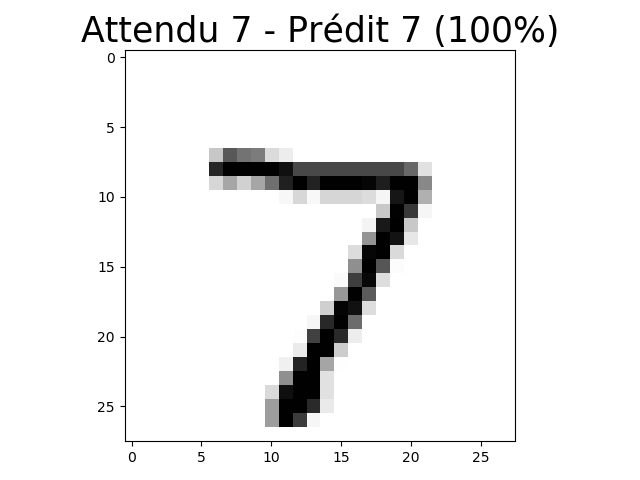
\includegraphics[scale=\myscale,scale=0.20]{figures/tfconv-chiffre-test-result-0}
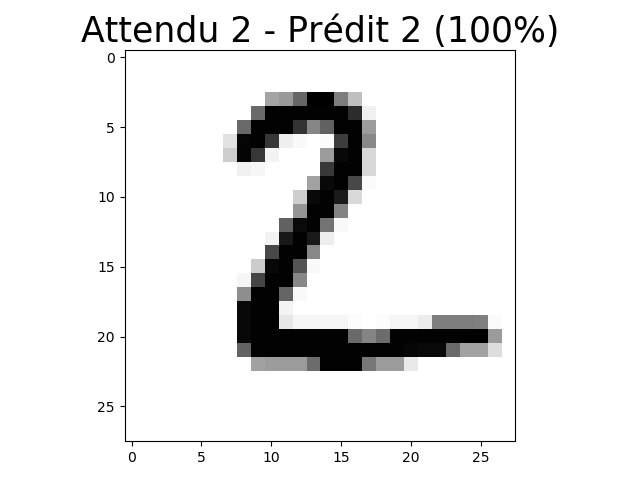
\includegraphics[scale=\myscale,scale=0.20]{figures/tfconv-chiffre-test-result-1}
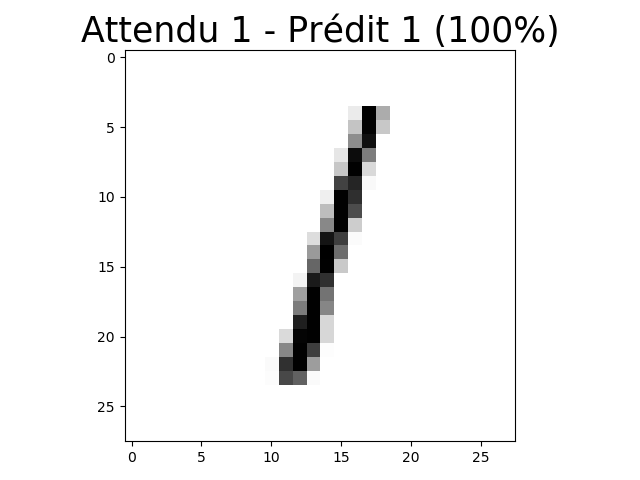
\includegraphics[scale=\myscale,scale=0.20]{figures/tfconv-chiffre-test-result-2}
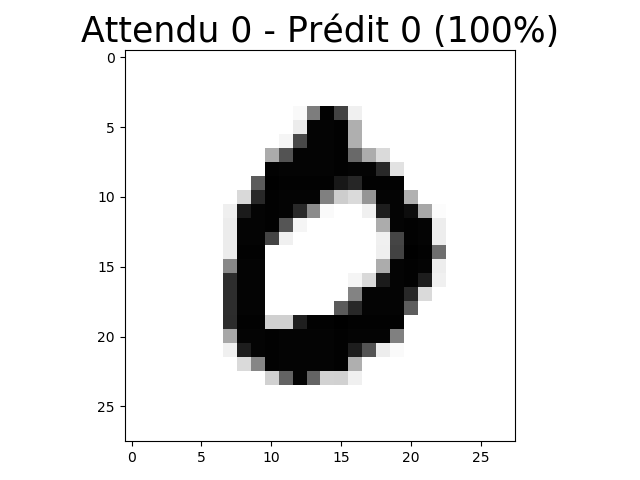
\includegraphics[scale=\myscale,scale=0.20]{figures/tfconv-chiffre-test-result-3}
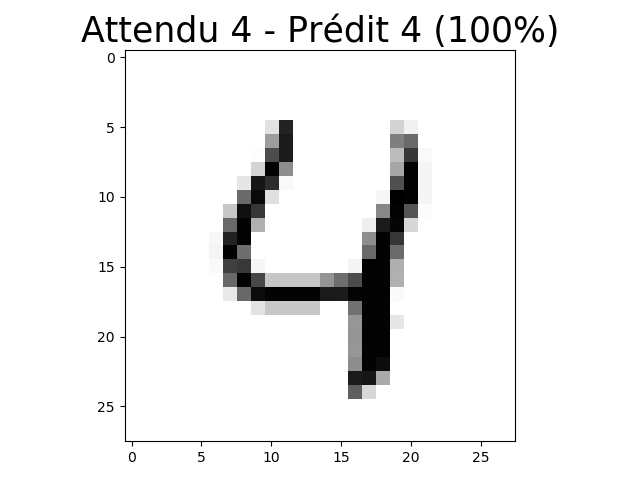
\includegraphics[scale=\myscale,scale=0.20]{figures/tfconv-chiffre-test-result-4}
\end{center}
\begin{center}
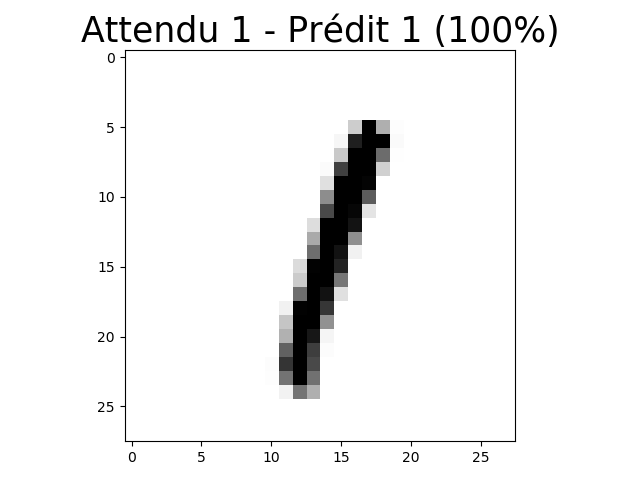
\includegraphics[scale=\myscale,scale=0.20]{figures/tfconv-chiffre-test-result-5}
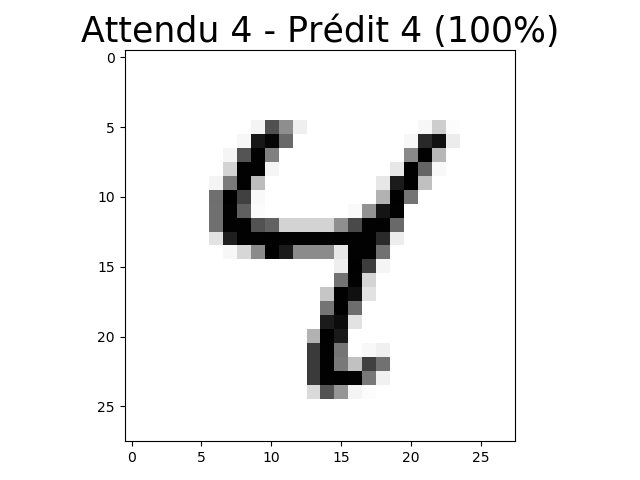
\includegraphics[scale=\myscale,scale=0.20]{figures/tfconv-chiffre-test-result-6}
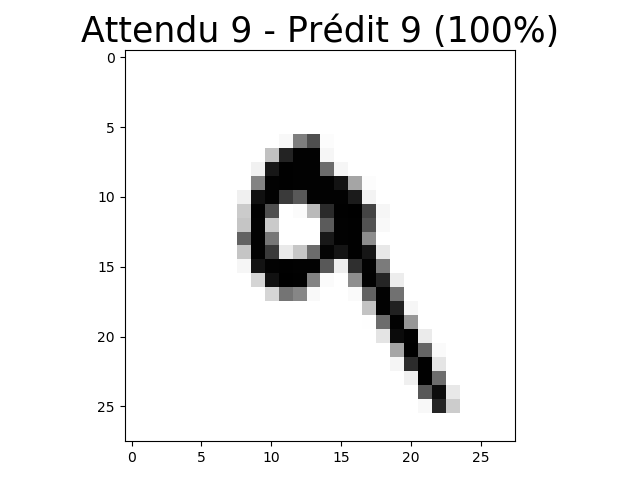
\includegraphics[scale=\myscale,scale=0.20]{figures/tfconv-chiffre-test-result-7}
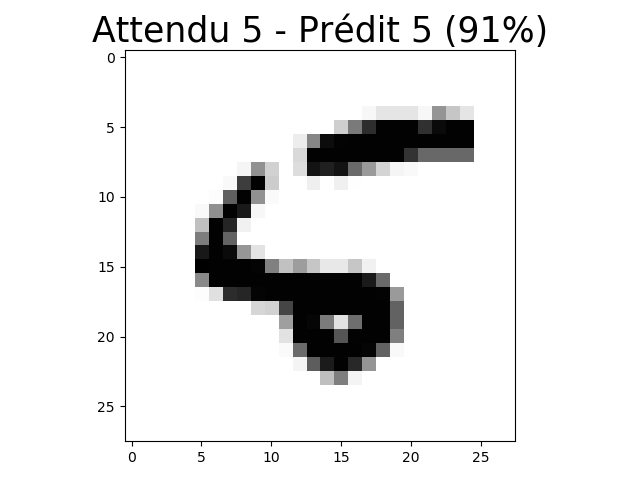
\includegraphics[scale=\myscale,scale=0.20]{figures/tfconv-chiffre-test-result-8}
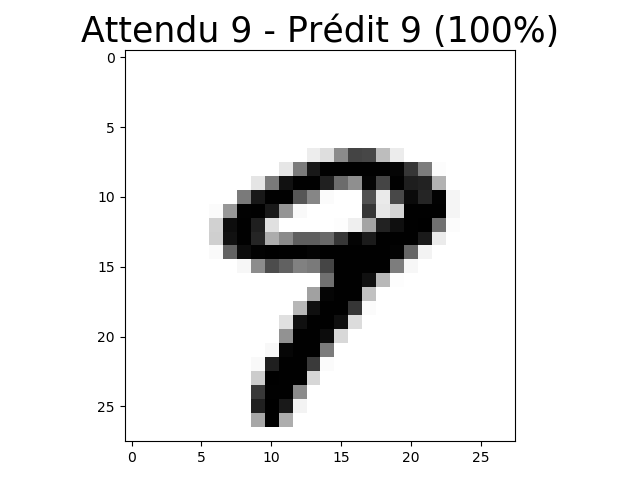
\includegraphics[scale=\myscale,scale=0.20]{figures/tfconv-chiffre-test-result-9}
\end{center}

Sur les exemples ci-dessus toutes les prédictions sont correctes avec en plus une quasi-certitude de $100\%$, à l'exception de l'avant-dernière image qui conduit à une bonne prédiction mais avec une certitude plus faible.
En effet le vecteur de sortie pour cette image est :
$$Y = (0, 0, 0, 0, 0, 0.911, 0.089, 0, 0, 0).$$
Le chiffre $5$ est donc prédit à $91\%$ avec un léger doute avec le chiffre $6$ à $9\%$, ce qui est tout à fait rassurant vu que ce chiffre est très mal dessiné !



%%%%%%%%%%%%%%%%%%%%%%%%%%%%%%%%%%%%%%%%%%%%%%%%%%%%%%%%%%%%%%%%%%%%%
\section{Reconnaissance d'images}

On souhaite reconnaître des objets ou des animaux sur de petites photos.

%--------------------------------------------------------------------
\subsection{Données}

On rappelle que la base CIFAR-10\index{donnees@données!CIFAR-10}, déjà rencontrée dans le chapitre \og{}Python : tensorflow avec keras - partie 2\fg{} contient $50\,000$ images d'apprentissage, réparties en $10$ catégories.

\begin{center}
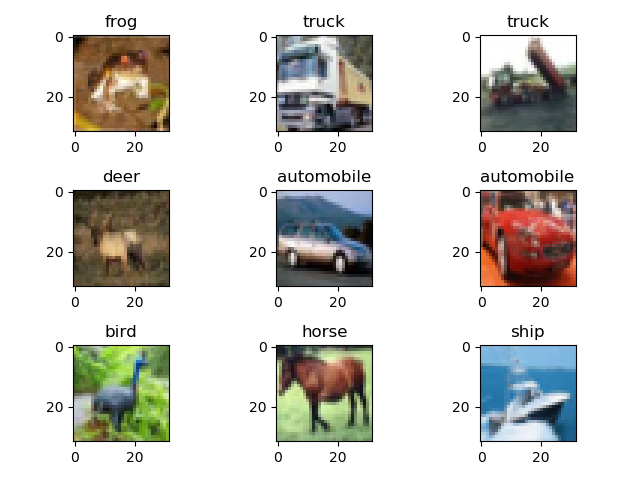
\includegraphics[scale=\myscale,scale=0.7]{figures/tfconv-images-train}
\end{center}

Chaque image possède $32\times 32$ pixels de couleurs. Une entrée correspond donc à un tableau
$(32,32,3)$.

\myfigure{0.5}{
\tikzinput{fig-tfconv-cnn-07}
}   

%--------------------------------------------------------------------
\subsection{Modèle}

L'architecture du réseau utilisé est composée de plusieurs couches de convolution.
Pour diminuer le nombre de poids à calculer, on intercale des couches de pooling (regroupement de termes). Ces pooling sont des max-pooling de taille $2 \times 2$.
De tels regroupements divisent par $4$ la taille des données en conservant les principales caractéristiques, ce qui fait que la couche de neurones suivante possèdera $4$ fois moins de poids à calculer.
 
\myfigure{0.28}{
\tikzinput{fig-tfconv-cnn-08}
}  
 
\myfigure{0.4}{
\tikzinput{fig-tfconv-bloc-02}
}  
 
Il y a en tout $153\,546$ poids à calculer. 
Sans les deux couches de pooling, il y aurait $767\,946$ poids.

%--------------------------------------------------------------------
\subsection{Programme}

\begin{lstlisting}
modele = Sequential()

# Première couche de convolution : 64 neurones, motif 3x3, activ. relu
modele.add(Conv2D(64, kernel_size=3, padding='same', activation='relu',
                      input_shape=(32,32,3)))

# Deuxième couche de convolution : 64 neurones
modele.add(Conv2D(64, kernel_size=3, padding='same', activation='relu'))

# Mise en commun (pooling)
modele.add(MaxPooling2D(pool_size=(2, 2)))

# Troisième couche de convolution : 64 neurones
modele.add(Conv2D(64, kernel_size=3, padding='same', activation='relu'))

# Mise en commun (pooling)
modele.add(MaxPooling2D(pool_size=(2, 2)))

# Quatrième couche de convolution : 64 neurones
modele.add(Conv2D(64, kernel_size=3, padding='same', activation='relu'))

# Aplatissage 
modele.add(Flatten())

# Couche de sortie : 1O neurones
modele.add(Dense(10, activation='softmax'))
\end{lstlisting}

%--------------------------------------------------------------------
\subsection{Explications}

La nouveauté est ici l'ajout de couches de pooling par la commande :
\mycenterline{\ci{modele.add(MaxPooling2D(pool_size=(2, 2)))}}
\index{tf@\tensorflow/\keras!MaxPooling2D@\ci{MaxPooling2D()}}

%--------------------------------------------------------------------
\subsection{Résultats}

Après une dizaine d'époques, on obtient plus de $80\%$ de précision sur les données d'entraînement et un peu moins de $75\%$ sur les données de test. Ainsi les trois quarts des images sont correctement prédites.

\begin{center}
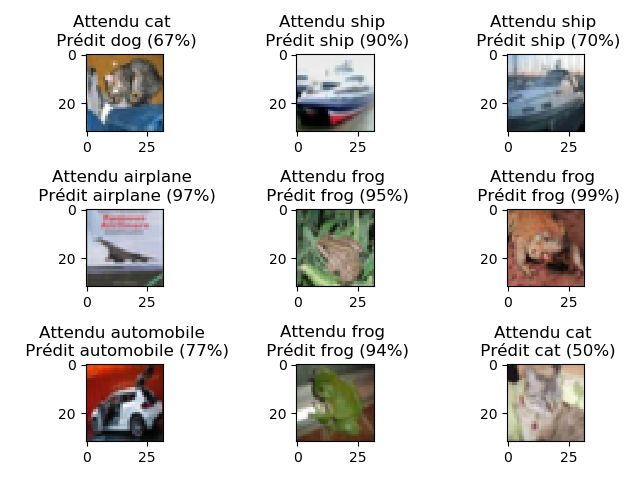
\includegraphics[scale=\myscale,scale=0.8]{figures/tfconv-images-test}
\end{center}



%%%%%%%%%%%%%%%%%%%%%%%%%%%%%%%%%%%%%%%%%%%%%%%%%%%%%%%%%%%%%%%%%%%%%
\section{Chat vs chien}

Il s'agit de décider si une photo est celle d'un chat ou d'un chien.

%--------------------------------------------------------------------
\subsection{Données}

Nous allons traiter une situation plus réaliste que celles vues jusqu'ici, car les données sont de \og{}vraies\fg{} photos qu'il faut préparer avant de commencer les calculs.

\textbf{Récupérer les données.}

Télécharger les données sur le site \og{}Kaggle\fg{} qui a organisé un concours de reconnaissance de photos :
\mycenterline{\href{https://www.kaggle.com/c/dogs-vs-cats/data}{https://www.kaggle.com/c/dogs-vs-cats/data}}
Le fichier à récupérer est \og{}train.zip\fg{} ($600$ Mo).

\textbf{Les photos.}
Le fichier contient $25\,000$ photos couleurs de différentes tailles :
\begin{itemize} 
  \item $12\,500$ photos de chats, nommées sous la forme \ci{cat.1234.jpg},
  \item $12\,500$ photos de chiens, nommées sous la forme \ci{dog.1234.jpg}.    
\end{itemize}

\begin{center}
\begin{minipage}{0.45\textwidth}
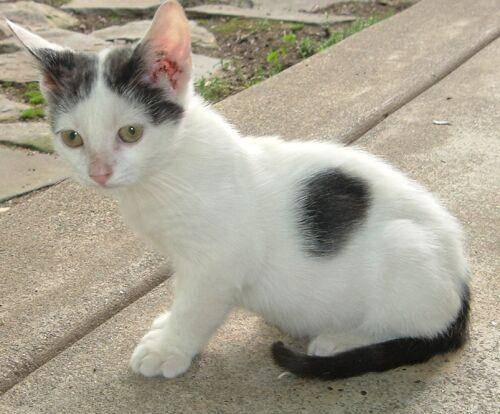
\includegraphics[scale=\myscale,scale=0.3]{figures/cat_3}
\end{minipage}
\begin{minipage}{0.45\textwidth}
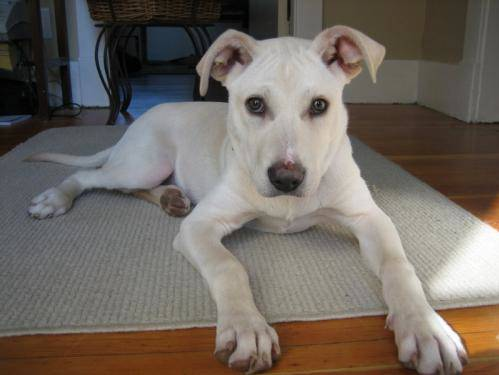
\includegraphics[scale=\myscale,scale=0.34]{figures/dog_87}
\end{minipage}
\end{center}

\textbf{Organiser les photos.}
Répartir à la main les photos dans des sous-répertoires avec la structure suivante :
\begin{lstlisting}
  donnees/
      train/
          cats/
          dogs/
      test/
          cats/
          dogs/
\end{lstlisting}

Déplacer $10\,000$ photos de chats dans \ci{donnees/train/cats} 
 puis $10\,000$ photos de chiens dans \ci{donnees/train/dogs}.
Déplacer les $2\,500$ photos de chats restantes  dans \ci{donnees/test/cats}
puis les $2\,500$ photos de chiens restantes dans \ci{donnees/test/dogs}.

Note : vous pouvez commencer avec seulement $1\,000$ photos par sous-répertoire pour des calculs plus rapides.

\textbf{Redimensionnement des photos.}
Les photos vont toutes être redimensionnées à la même taille, par exemple $64 \times 64$.
Ces tâches préliminaires seront effectuées pour nous par \keras.
De plus, comme les photos représentent une grande quantité de données, nous allons voir comment \keras{} permet de ne mettre en mémoire qu'une petite quantité d'images à chaque étape de la descente de gradient.


\begin{center}
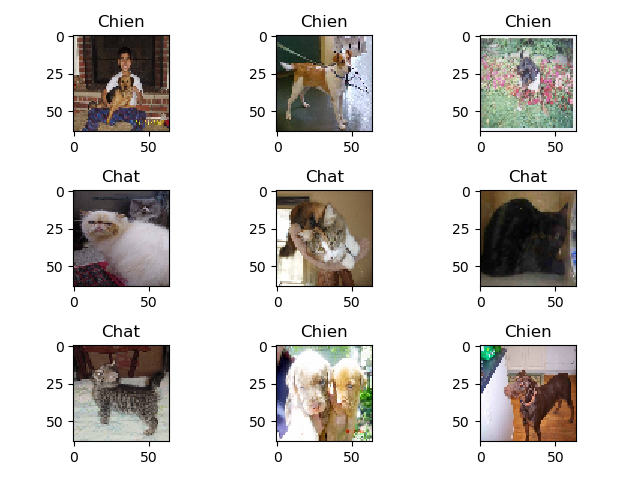
\includegraphics[scale=\myscale,scale=0.8]{figures/tfconv-chienchat-train}
\end{center}


%--------------------------------------------------------------------
\subsection{Modèle}

On alterne : couche de convolution, pooling et dropout.
Il y a $206\,685$ poids à calculer.

\myfigure{0.35}{
\tikzinput{fig-tfconv-bloc-03}
} 


%--------------------------------------------------------------------
\subsection{Programme}

\begin{lstlisting}
import numpy as np
from tensorflow import keras
from tensorflow.keras import optimizers
from tensorflow.keras.models import Sequential
from tensorflow.keras.layers import Dense,Conv2D,Flatten,MaxPooling2D,Dropout
from tensorflow.keras.preprocessing.image import ImageDataGenerator

# Partie A. Données

# A télécharger sur https://www.kaggle.com/c/dogs-vs-cats/data
train_directory = 'monrepertoire/donnees/train'
test_directory  = 'monrepertoire/donnees/test'
image_width = 64
image_height = 64
nb_train_images = 20000

# Transforme les images en données d'apprentissage : 
# (a) reformate les images en taille unique, 
# (b) créé une classification (à partir de chaque sous-répertoire) 
# 0 pour les chats  et 1 pour les chiens 
train_datagen = ImageDataGenerator(rescale =1./255)
training_set = train_datagen.flow_from_directory(train_directory,
                                       target_size=(image_width,image_height),
                                       batch_size= 32,
                                       shuffle=True, seed=13,
                                       class_mode='binary')

# Partie B. Réseau 
modele = Sequential()

modele.add(Conv2D(64, kernel_size=3, padding='same', activation='relu', 
                      input_shape=(image_width,image_height,3)))
modele.add(MaxPooling2D(pool_size=(2, 2)))
modele.add(Dropout(0.5))

modele.add(Conv2D(64, kernel_size=3, padding='same', activation='relu'))
modele.add(MaxPooling2D(pool_size=(2, 2)))
modele.add(Dropout(0.5))

modele.add(Conv2D(64, kernel_size=3, padding='same', activation='relu'))
modele.add(MaxPooling2D(pool_size=(2, 2)))
modele.add(Dropout(0.5))

modele.add(Flatten())
modele.add(Dense(32, activation='relu'))
modele.add(Dense(1, activation='sigmoid'))

modele.compile(loss='binary_crossentropy',
               optimizer='adam',
               metrics=['accuracy'])

# Partie C. Apprentissage
history = modele.fit_generator(training_set,
                        steps_per_epoch = nb_train_images // 32,
                        epochs = 10)

\end{lstlisting}

%--------------------------------------------------------------------
\subsection{Explications}

La nouveauté est ici l'ajout de couches de dropout par la commande :
\mycenterline{\ci{modele.add(Dropout(0.5))}}

\index{tf@\tensorflow/\keras!Dropout@\ci{Dropout()}}

%--------------------------------------------------------------------
\subsection{Résultats}

Après pas mal de calculs et une quarantaine d'époques, on obtient une précision de $85\%$, ce qui est tout fait correct, même si on est loin des $99\%$ de précision des meilleurs résultats du concours \og{}Kaggle\fg{}. \`A vous de jouer !

\begin{center}
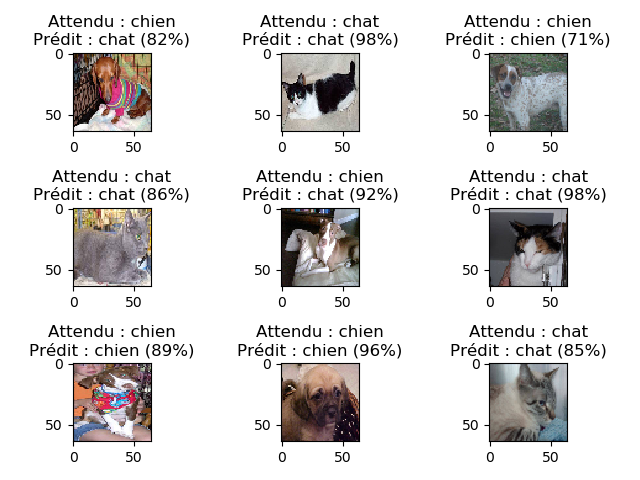
\includegraphics[scale=\myscale,scale=0.9]{figures/tfconv-chienchat-test}
\end{center}

On montre ci-dessus des images de test avec deux photos mal identifiées, peut-être à cause d'éléments extérieurs (le gilet coloré en haut à gauche, la serviette au milieu).




%%%%%%%%%%%%%%%%%%%%%%%%%%%%%%%%%%%%%%%%%%%%%%%%%%%%%%%%%%%%%%%%%%%%%
\section{Que voit un réseau de neurones ?}

Une des difficultés des réseaux de neurones est qu'ils agissent comme une \og{}boîte noire\fg{}. Une fois bien paramétrés, ils répondent efficacement à un problème. Mais même avec plus $99\%$ de bonnes décisions, l'utilisateur peut avoir un doute sur la réponse donnée par une machine (en particulier pour une question médicale, la conduite autonome\ldots). Il est donc intéressant d'inspecter le fonctionnement interne d'un réseau déjà paramétré en essayant de comprendre ce que font les couches intermédiaires.


%--------------------------------------------------------------------
\subsection{Un exemple}

On reprend l'exemple de la reconnaissance de chiffres manuscrits de la base MNIST.\index{donnees@données!MNIST} On construit un réseau simple :
\begin{itemize}
  \item \textbf{Entrée.} Une image en niveau de gris de taille $28\times 28$.
  \item \textbf{Couche 1.} Une couche de convolution avec $16$ filtres (autrement dit $16$ sous-couches).
  \item \textbf{Couche 2.} Une autre couche de convolution avec encore $16$ filtres.
  \item \textbf{Couche 3.} Une couche de max-pooling $2\times2$.
  \item \textbf{Aplatissement.} 
  \item \textbf{Couche dense et sortie.} Une couche dense de  $10$ neurones qui est aussi la couche de sortie.
\end{itemize}

\myfigure{0.34}{
\tikzinput{fig-tfconv-cnn-06}
} 

On entraîne le réseau sur plusieurs époques jusqu'à ce qu'il prédise correctement $99\%$ des images de test.
Nous allons visualiser l'action des couches 1, 2 et 3.


%--------------------------------------------------------------------
\subsection{Visualisation de couches}

\textbf{Première couche.}
Voici ce que \og{}voit\fg{} le réseau à la sortie de la couche 1, tout d'abord avec un exemple où l'entrée est un chiffre $4$.
\begin{center}
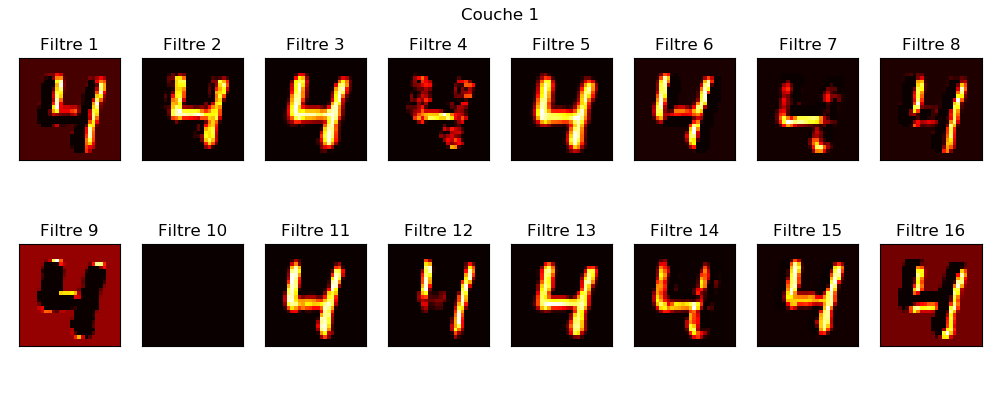
\includegraphics[scale=\myscale,scale=0.65]{figures/tfconv-viz2-n56-4-c1}
\end{center}
La couleur d'un pixel représente la valeur de la sortie d'un neurone de convolution (blanc/élevée, noir/faible). Comme il y a $16$ sous-couches cela donne $16$ images différentes pour le même chiffre $4$. 

Les filtres ont différentes actions et certaines peuvent être déterminées. Par exemple, il semble que les filtres 1 et 8 mettent en avant les lignes verticales, alors que les filtres 4 et 7 renforcent les lignes horizontales. Le filtre 16 effectue une sorte de mise en relief. D'autres sont difficiles à interpréter.

Voici l'action de la même couche 1 sur un autre chiffre.  

\begin{center}
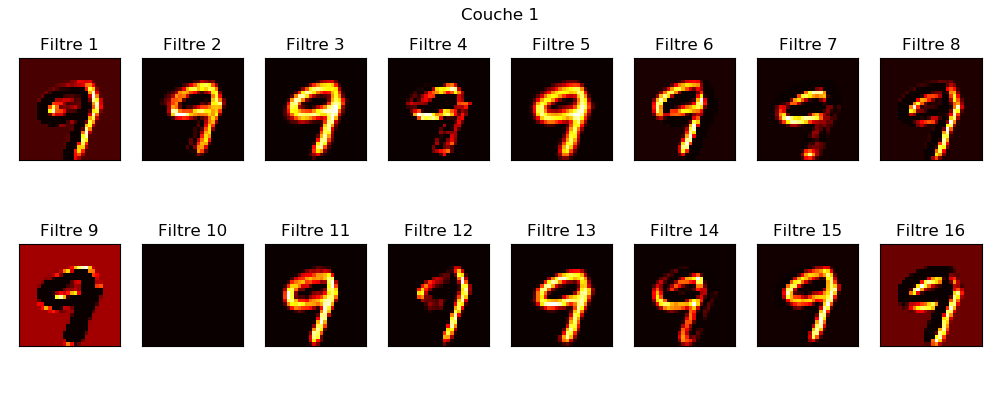
\includegraphics[scale=\myscale,scale=0.65]{figures/tfconv-viz2-n58-9-c1}
\end{center}

\bigskip
\textbf{Deuxième couche.}
Voyons maintenant ce qu'il se passe à la sortie de la couche 2, pour notre chiffre 4 et notre chiffre 9.
Attention les filtres sont de nouveau numérotés de 1 à 16 mais n'ont rien à voir avec les filtres de la couche 1.

\begin{center}
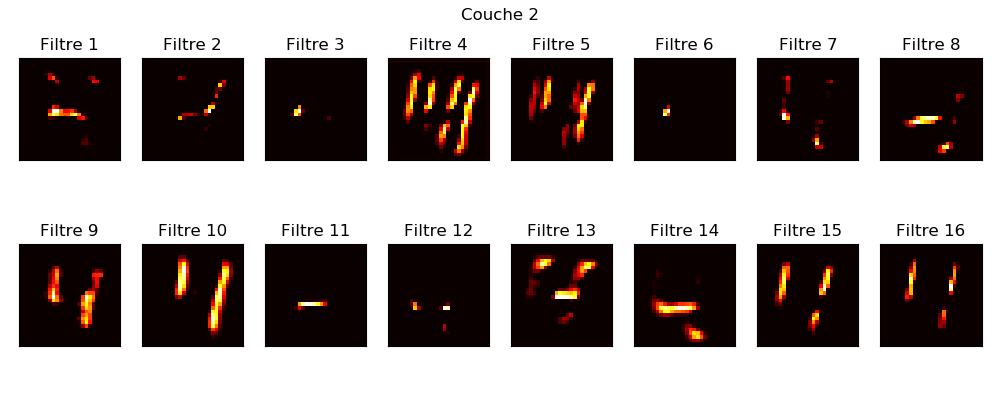
\includegraphics[scale=\myscale,scale=0.65]{figures/tfconv-viz2-n56-4-c2}
\end{center}

\begin{center}
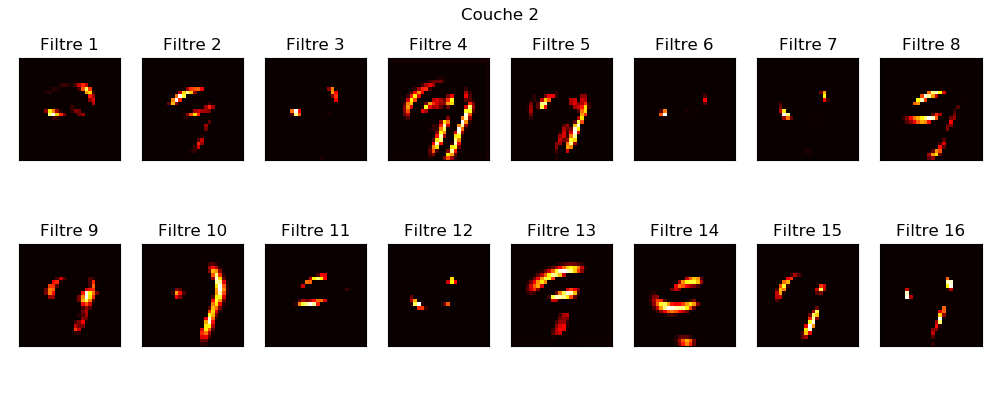
\includegraphics[scale=\myscale,scale=0.65]{figures/tfconv-viz2-n58-9-c2}
\end{center}

La deuxième couche renvoie une vision plus abstraite de nos chiffres et les distingue. Par exemple le filtre 11 différencie le chiffre 4 (un seul trait horizontal) du chiffre 9 (deux traits horizontaux), de même avec le filtre 10 et ses traits verticaux.

\bigskip
\textbf{Troisième couche.}
C'est une couche de max-pooling. Cette fois les filtres de la couche 3 correspondent aux filtres le couche 2. Même si les tailles sont réduites d'un facteur $2\times2$, on voit sur l'exemple du chiffre 4 ci-dessous que les principales caractéristiques sont conservées.

\begin{center}
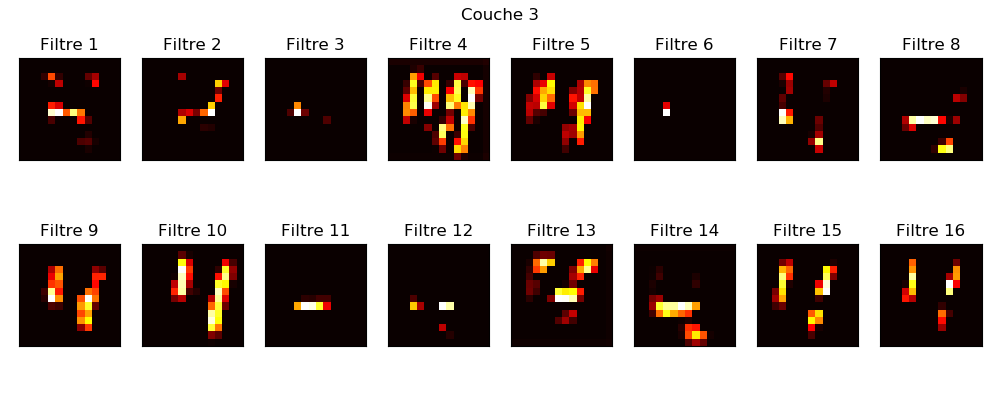
\includegraphics[scale=\myscale,scale=0.65]{figures/tfconv-viz2-n56-4-c3}
\end{center}


%--------------------------------------------------------------------
\subsection{Visualisation de filtres}

Un autre point de vue est de se concentrer sur un seul filtre d'une seule couche et de regarder comment celui-ci traite différentes images.


\textbf{Première couche.}
Voici deux exemples pour la couche 1 : le filtre 12 qui met en évidence les segments verticaux et le filtre 16 qui met en relief.
\begin{center}
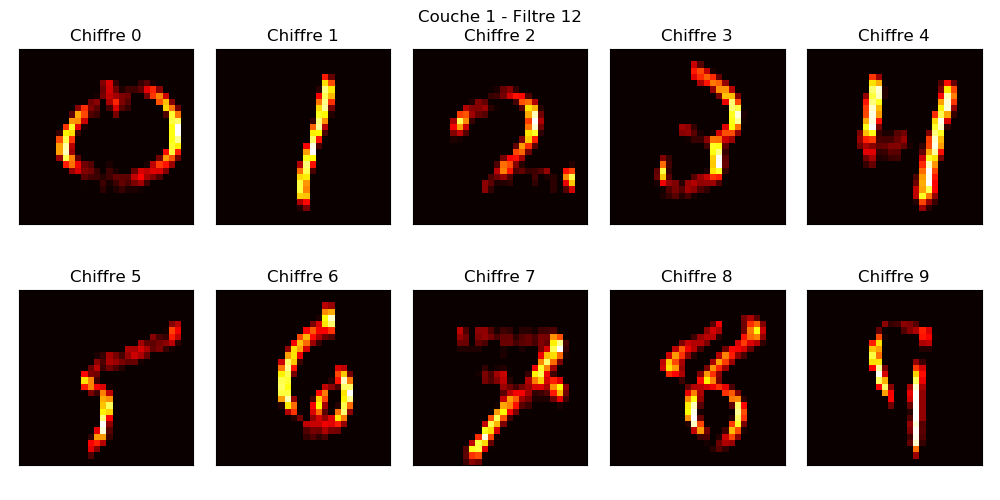
\includegraphics[scale=\myscale,scale=0.5]{figures/tfconv-viz3-c1-f12}
\end{center}

\begin{center}
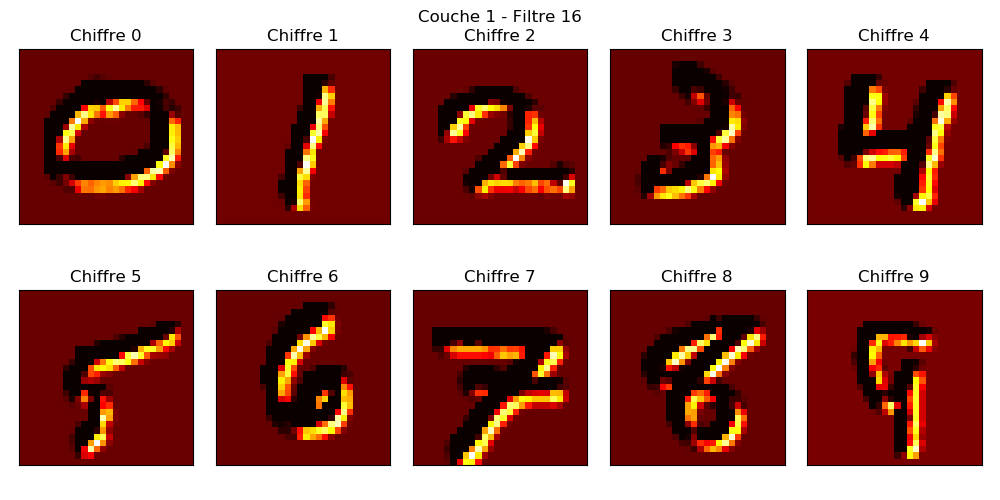
\includegraphics[scale=\myscale,scale=0.5]{figures/tfconv-viz3-c1-f16}
\end{center}

\bigskip
\textbf{Deuxième couche.}
Le filtre 10 renforce les lignes verticales. Le filtre 14 renforce les lignes horizontales, on voit ainsi qu'il permet de détecter le chiffre 1, c'est le seul chiffre qui n'active (presque) aucun pixel pour ce filtre. (On rappelle que les filtres de cette deuxième couche n'ont rien à voir avec les filtres de la première couche.)

\begin{center}
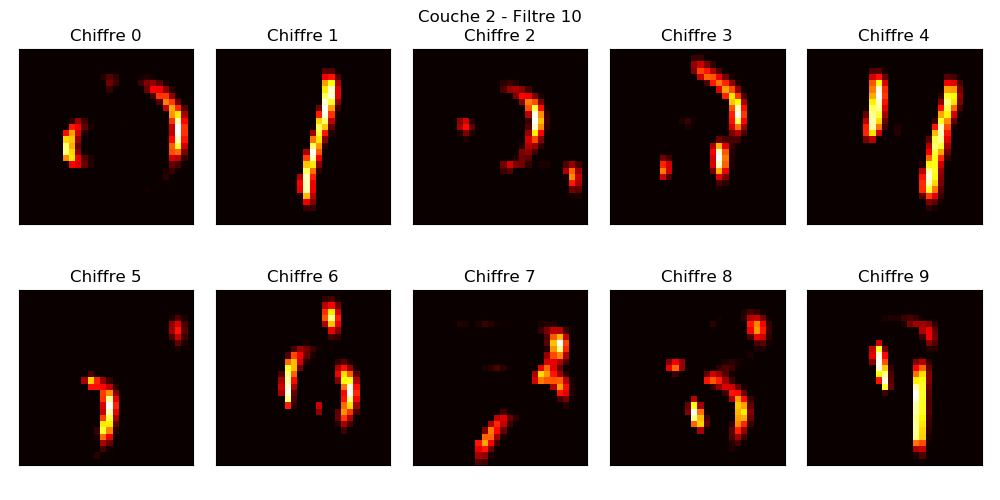
\includegraphics[scale=\myscale,scale=0.5]{figures/tfconv-viz3-c2-f10}
\end{center}

\begin{center}
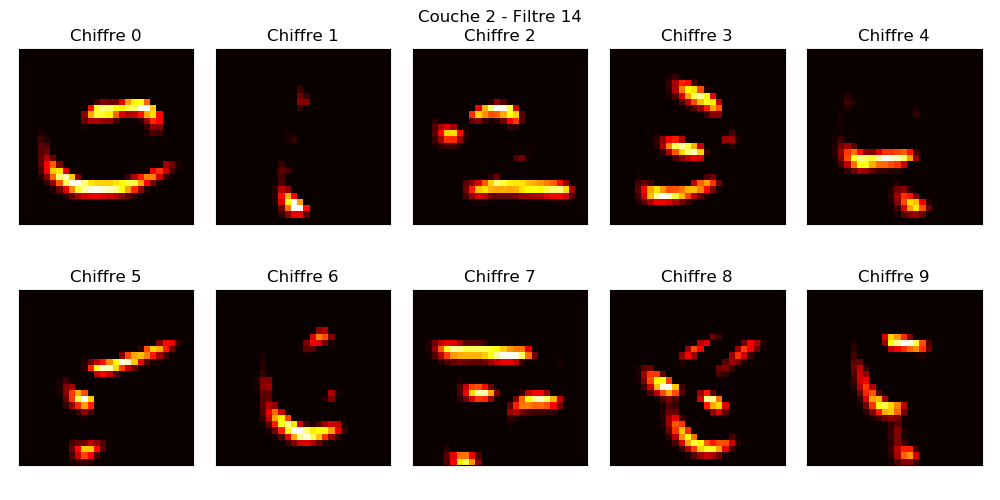
\includegraphics[scale=\myscale,scale=0.5]{figures/tfconv-viz3-c2-f14}
\end{center}

\bigskip
\textbf{Troisième couche.}
La troisième couche est une couche de pooling, ainsi ses filtres correspondent aux filtres de la couche précédente. 

\begin{center}
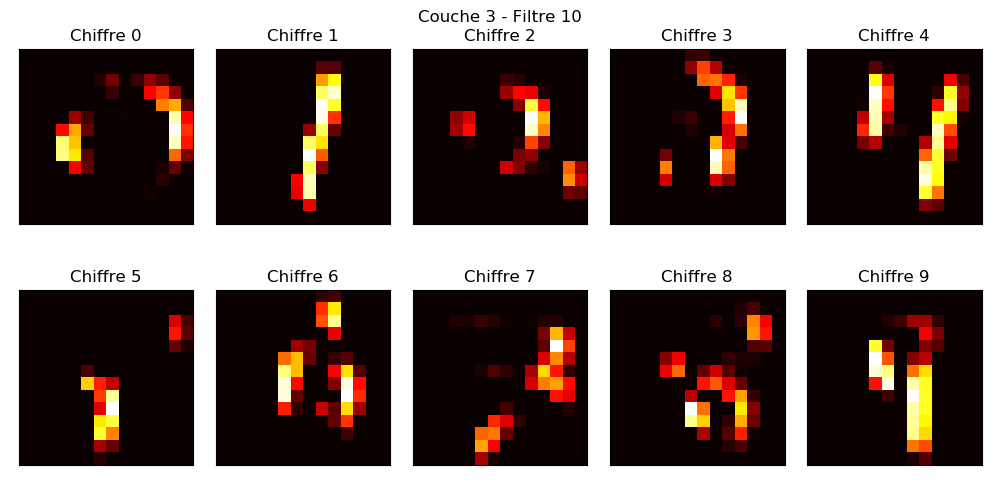
\includegraphics[scale=\myscale,scale=0.5]{figures/tfconv-viz3-c3-f10}
\end{center}

\begin{center}
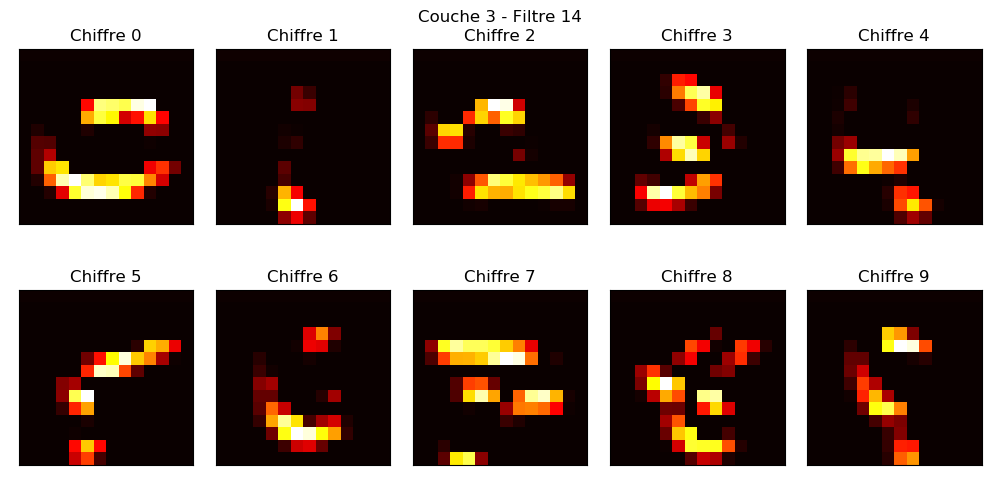
\includegraphics[scale=\myscale,scale=0.5]{figures/tfconv-viz3-c3-f14}
\end{center}
\end{document}
